\documentclass[a4paper,12pt]{article}
\usepackage{amsmath,amssymb,amsfonts,amsthm}
\usepackage{tikz}
\usepackage[utf8x]{inputenc}
\usepackage[T2A]{fontenc} 
\usepackage[russian]{babel}
\usepackage{cmap} 
\usepackage{ gensymb }
% Так ссылки в PDF будут активны
\usepackage[unicode]{hyperref}
\usepackage{ textcomp }
\usepackage{indentfirst}
\usepackage[version=3]{mhchem}

% вы сможете вставлять картинки командой \includegraphics[width=0.7\textwidth]{ИМЯ ФАЙЛА}
% получается подключать, как минимум, файлы .pdf, .jpg, .png.
\usepackage{graphicx}
% Если вы хотите явно указать поля:
\usepackage[margin=1in]{geometry}
% Или если вы хотите задать поля менее явно (чем больше DIV, тем больше места под текст):
% \usepackage[DIV=10]{typearea}

\usepackage{fancyhdr}

\newcommand{\bbR}{\mathbb R}%теперь вместо длинной команды \mathbb R (множество вещественных чисел) можно писать короткую запись \bbR. Вместо \bbR вы можете вписать любую строчку букв, которая начинается с '\'.
\newcommand{\eps}{\varepsilon}
\newcommand{\bbN}{\mathbb N}
\newcommand{\dif}{\mathrm{d}}

\newtheorem{Def}{Определение}


\pagestyle{fancy}
\makeatletter % сделать "@" "буквой", а не "спецсимволом" - можно использовать "служебные" команды, содержащие @ в названии
\fancyhead[L]{\footnotesize }%Это будет написано вверху страницы слева
\fancyhead[R]{\footnotesize ФУПМ МФТИ}
\fancyfoot[L]{\footnotesize \@author}%имя автора будет написано внизу страницы слева
\fancyfoot[R]{\thepage}%номер страницы —- внизу справа
\fancyfoot[C]{}%по центру внизу страницы пусто

\renewcommand{\maketitle}{%
	\noindent{\bfseries\scshape\large\@title\ \mdseries\upshape}\par
	\noindent {\large\itshape\@author}
	\vskip 2ex}
\makeatother
\def\dd#1#2{\frac{\partial#1}{\partial#2}}


\title{10.4 \\ Магнитные моменты легких ядер}
\author{Северилов Павел, 674} 
\date{08 октября 2018 г.}

\begin{document}
		\maketitle
		\section*{Теория}
		
		
		Отношение $\gamma$ магнитного момента к механическому называется гиромагнитным отношением:
		\begin{equation}
		\vec{\mu} = \gamma \vec{M}.
		\end{equation}
		Величину $\gamma$ также можно записать в виде произведения: $$\gamma = g\gamma_0,$$ где $g$ -- фактор Ланде, а $\gamma_0  = -\dfrac{e_0}{2m_ec}$ -- гиромагнитное отношение для орбитального движения электрона в атоме.\\
		Зачастую, вместо $\gamma$ используют более простую величину - $g$-фактор. Он также является отношением магнитного момента к механическому, но при этом магнитный момент измеряется в ядерных магнетонах Бора ($\mu_\text{я} = e \hbar / 2 m_p c$), а механический момент -- в единицах $\hbar$:
		\begin{equation}
		g = \frac{\mu / \mu _\text{я}}{M/\hbar} = \frac{\mu}{\mu_\text{я}} \frac{\hbar}{M} = \frac{\hbar}{\mu_\text{я}} \gamma.
		\end{equation}
		Отсюда 
		\begin{equation} \label{mu}
		\vec{\mu} = \frac{\mu_\text{я}}{\hbar} g \vec{M}.
		\end{equation}
		
		
		Проецируя $M$ и $\mu$ на направление вектора $B$, получаем:
		\begin{equation}
		\vec{\mu_B} = \frac{\mu_\text{я}}{\hbar} g \vec{M_B} = \mu_\text{я} g m.
		\end{equation}
		Наибольшее значение $\mu_B$ равно $\mu_\text{я} g I$. Его принято называть магнитным моментом ядра. 
		
		Расстояние между двумя соседними компонентами расщепившегося в магнитном поле уровня:
		\begin{equation} \label{deltaE}
		\Delta E = B \Delta \mu_B = B \mu_\text{я} g \Delta m = B \mu_\text{я} g.
		\end{equation}
		~
		Между компонентами расщепившегося уровня могут происходить электромагнитные переходы. Энергия квантов при этом определяется выражением (\ref{deltaE}), и явление носит резонансный характер. Частота излучения:
		
		\begin{equation} \label{nu}
		\nu = \frac{\Delta E}{h} = \frac{B \mu_\text{я} g}{h}.
		\end{equation}
		
		Возбуждение переходов между компонентами расщепившегося ядерного уровня - ядерный магнитный резонанс (ЯМР). 
		
		
		~
		В данной работе $g$-фактор определяется с помощью явления ЯМР. Изменяя частоту переменного магнитного поля, мы можем найти положение максимума поглощения, т.е. частоту резонанса. По этому максимуму определяется $g$-фактор из соотношения (\ref{nu}).
		\newpage
		\section*{Установка}
		\begin{figure}[ht!]
			\centering
			{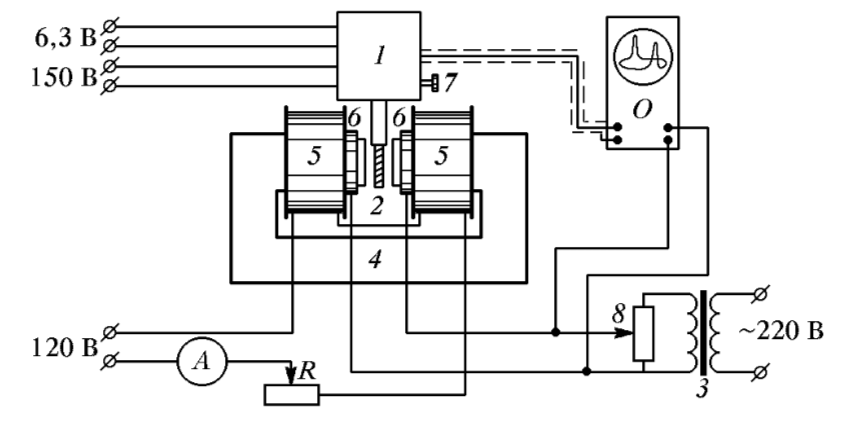
\includegraphics[width=0.6\linewidth]{scheme.png}}
			\caption{Схема установки: 1 - часть индикаторной установки, исследуемый образец,3 - трансформатор,4 - электромагнит, 5 - катушки, 6 - модулирующие катушки, 8 - потенциометр }
		\end{figure}
		Различие между двумя соседними компонентами определяется формулой $$\Delta E = g\mu_{\text{я}}B_0,$$ а соответствующая частота находится как $f_0 = \dfrac{\Delta E}{h} = \dfrac{g\mu_{\text{я}}B_0}{h}$.
		\section*{Задания}
		Помещая разные образцы между полюсами электромагнита и устанавливая частоту $f_0$ индикаторной установки в диапазоне $1\div20$ МГц, плавно меняли магнитное поле в зазоре электромагнита, пока не обнаруживали сигнал ЯМР.
		
		Полученные данные приведены в таблице:
		
		\begin{table} [h]
			\centering
			\caption{Полученные данные для разных образцов}
			\begin{tabular}{|l||c|c|}
				\hline
				Образец  & Вода & Резина \\
				\hline
				$f$, МГц & 9,62 & 9,80 \\
				\hline
				$B$, мТл & 226 & 230 \\
				\hline
			\end{tabular}
		\end{table}
		
		По полученным данным определим $g-$факторы исследуемых ядер по следующей формуле:
		
		\begin{equation}
		g_\text{я} = \frac{\hbar \omega_0}{\mu_\text{я} B_0} = \frac{h f_0}{\mu_\text{я} B_0}
		\end{equation}
		
		Учитывая, что угловой момент протона определяется только его спином, рассчитали магнитный момент протона по формуле:
		
		\begin{equation}
		\mu = g_\text{я} \mu_\text{я}I
		\end{equation}

		\newpage
		Из рассчитанных данных получили таблицу:
		
		
		\begin{table} [h]
			\centering
			\caption{Обработанные данные} 
			\begin{tabular}{|l||c|c|c|c|c|}
				\hline
				Образец & $I$ & $g_\text{я}$ & $g_\text{я, табл.}$ & $\mu$ $(\text{в} ~\mu_\text{я})$ & $ \mu_\text{табл.}, \mu_\text{я} $ \\
				\hline
				1. Протон (резина)  & 0,5 & 5,57 & 5,58 & 2,785 & 2,79  \\
				\hline
				2. Протон (вода)& 0,5 & 5,58 & 5,58 & 2,79 & 2,79  \\
				\hline
			\end{tabular}
		\end{table}
	
		\section*{Вывод}
		
		В работе мы экспериментально, методом ядерного магнитного резонанса, нашли магнитный момент ядра протона и его g-фактор. Полученные значения хорошо соотносятся с табличными.

\end{document}
